\documentclass[sigplan,10pt,screen]{acmart}
\renewcommand\footnotetextcopyrightpermission[1]{}
\pagestyle{plain}

\usepackage{datetime}
\usepackage{url}
\usepackage{hyperref}
\usepackage{xspace}
\usepackage{amssymb}% http://ctan.org/pkg/amssymb
\usepackage{pifont}% http://ctan.org/pkg/pifont
\usepackage{todonotes}
\usepackage{cleveref}
\usepackage{tabularx}
\usepackage{booktabs}
\usepackage{multirow}
\usepackage{algorithm}
\usepackage[noend]{algpseudocode}
\usepackage{subcaption}

 \aboverulesep=0ex
 \belowrulesep=0ex
 
\crefformat{section}{\S#2#1#3}
\crefformat{subsection}{\S#2#1#3}
\crefformat{subsubsection}{\S#2#1#3}

\settopmatter{printacmref=false, printfolios=true, printccs=false}
\renewcommand\footnotetextcopyrightpermission[1]{}
\pagestyle{plain} 

\newcommand{\cmark}{\color{teal}\ding{51}}%
\newcommand{\xmark}{\color{red}\ding{55}}%

%\conferenceinfo{SOSP'17}{October 29--31, 2017, Shanghai, China}
%\copyrightyear{2017} 


% These only appear when the 'preprint' option is specified.
% Enabling these will cause the first page of the document to fail the 
% format check on HotCRP :-(
%\titlebanner{Under submission to SOSP 2017 - do not cite or distribute}
%\preprintfooter{Draft of {\currenttime}, \today{}}

% No date in title area.
\date{}

% Paper number and no. of pages as author
%\authorinfo{Paper \textbf{\#XX}}{NN pages}

\newcommand{\mycaption}[2]{\caption{\textbf{#1}. \textit{#2}}}
\newcommand{\sref}[1]{\S\ref{#1}}
\newcommand{\vheading}[1]{\vspace{0.05in}\noindent\textbf{#1}}
\newcommand{\viheading}[1]{\vspace{0.05in}\noindent\emph{#1}}
\newcommand{\vitem}[1]{\item\textbf{#1}}    
%\newcommand{\vb}[1]{\textbf{#1}}
\newcommand{\vb}[1]{\emph{#1}}
\newcommand{\fsync}{\texttt{fsync()}\xspace}
\newcommand{\etal}{\textit{et al.}\xspace}
\newcommand{\ie}{\textit{i.e.,}\xspace}
\newcommand{\eg}{\textit{e.g.,}\xspace}
\newcommand{\etc}{\textit{etc.}\xspace}
\newcommand*{\affmark}[1][*]{\textsuperscript{#1}}
\newcommand*{\affaddr}[1]{#1} % No op here. Customize it for different styles.


\usepackage{ifthen}
\newboolean{publicversion}
\setboolean{publicversion}{false}
\ifthenelse{\boolean{publicversion}}{
  \newcommand{\grumbler}[3]{}
}{
  \newcommand{\grumbler}[3]{\textcolor{#3}{\bf #1: #2}}
}

\newcommand{\vc}[1]{\grumbler{Vijay}{#1}{red}}
\newcommand{\DM}[1]{\grumbler{DM}{#1}{blue}}
\newcommand{\AT}[1]{\grumbler{AT}{#1}{orange}}

% Actual document begins below.
\begin{document}

\title{Model Checking Persistent Memory Indexes With State Space Exploration}

\author{
  {\rm Soujanya Ponnapalli}
  \enspace\\ 
  \affaddr{Verification and Synthesis of Cyber Physical Systems (CS-395T or ASE-396)\\
  University of Texas at Austin}\hspace{10pt}
} %end author

\begin{abstract}
The advent of the Storage Class Memory (SCM) that is fast and byte-addressable
  similar to the Random Access Memory (DRAM or SRAM) and is persistent like the
  SSDs and hard disks, has attracted researchers to develop efficient data
  structures for adopting this persistent memory. However building efficient
  data structures for persistent memory that allow concurrent accesses to the
  data is challenging for two main reasons:
  1) The caches and registers remain volatile and require applications to flush
  the data from the caches to the persistent memory for durability.
  2) The cache flush instructions are reordered with load and store instructions
  in accordance to the memory model of the persistent memory and require
  applications to place fences to enforce ordering between these instructions.
  As fence and flush instructions incur heavy performance penalty and are
  crucial for correctness, the application developers should not insert fences
  unless they are strictly required for correctness. This tradeof complicates
  the design of persistent memory data structures and makes it extremely hard to
  reason about their correctness.

This paper aims at model checking persistent memory data structures for
  correctness and crash consistency by building a \emph{PM-Checker}. PM-Checker
  verifies that the data structure does not allow any instruction reorderings
  that can corrupt the data, and checks that crashing the data structure at any
  random point in time will not leave the persisted data in an inconsistent
  state. Overall, this paper models the persistent memory, formulizes the
  specifications for correctness and crash consistency and verifies
  state-of-the-art persistent memory data structures.
\end{abstract}


\maketitle

%\section{Problem Definition}

%\section{Related Work}

This section describes the prior work that verifies indexes
by modeling instruction level reordering, using model checking.
Here, the work is referred as SPEC - "State-Space Exploration
for Concurrent Algorithms under Weak Memory Ordering".

\vheading{Goals}. First, SPEC identifies that many concurrent indexes
often use lock-free synchronization for good performance. As
these indexes are exposed to weak memory ordering, there are
subtle bugs in their implementation. SPEC uses model checkers
to find correctness violations in concurrent indexes. SPEC
describes its technique using a concurrent queue that allows
\texttt{enqueue()} operation to be concurrent with a
\texttt{dequeue()} operation.

\vheading{Weak memory ordering}. Next, SPEC summarizes the weak
memory model used for verifying the concurrent queue. Considering
$\prec_{P}$ represents the program order and $\prec_{M}$ represents
the instruction ordering seen by the memory, SPEC defines five
axioms to capture the ordering relations.\\
\textbf{(A1)} If x and y are two operations to the same memory address
and y is a store, if x $\prec_{P}$ y then x $\prec_{M}$ y.
\\
\textbf{(A2)} For all loads, any store operation that accesses the
same memory address as the load that is termed say \emph{seed(l)}),
is considered to work on the same address as the load.
\\
\textbf{(A3)} \emph{Seed(l)} is the maximal element with respect
to $\prec_{M}$ in the set of all stores accessing the same address
as the load \emph{l}.
\\
\textbf{(A4)} If x and y are separated by a fence,
x $\prec_{P}$ f $\prec_{P}$ y; and x and y satisfy the type of
fence - for example x and y are loads for a load-load fence,
then x $\prec_{M}$ y.
\\
\textbf{(A5)} If x $\prec_{P}$ y and x $\prec_{d}$ y, where 
$\prec_{d}$ represents a dependency like y reading the register
that is loaded by x, then x $\prec_{M}$ y.

To summarize, the relaxed memory ordering differs in two respects
from the sequential consistency model. First, operations of one
thread may be reordered, but respecting fences and data dependencies.
Second, the global memory order is a merge of the possibly
reordered local orderings as in sequential ordering.

\vheading{Concurrent algorithms}. To elaborate the proposed technique
for modeling relaxed memory ordering, SPEC uses the concurrent two-lock
concurrent implementation of a queue.

To see the sequences of the loads and stores generated by the queue
implementation, it is transformed into a high-level machine language.
The machine language obeys the restriction that each instruction induces
at most one load and store instruction. To infer the possible instruction
reorderings, they find the data-dependencies between them.

\vheading{State space exploration}. Using the data dependencies,
a Promela model is deduced. The Promela model by construction can
execute the instructions with possible reorderings.
%\pagebreak
%\section{WORT}

This section describes WORT~\cite{201600}, write-optimized
radix tree. WORT is used in the rest of this work to describe
the modeling of PM behavior and to verifying consistency properties.

\vheading{Radix tree}. Several B-tree based indexing structures
have been proposed for PM. These indexes focused on reducing the
number of calls to the expensive memory fence and cache line flush
instructions. They employ an append-only update strategy. However,
these indexes require logging.

The first contribution of WORT is showing the appropriateness of radix
trees for indexing PM. As radix trees are structured around key prefixes,
key comparisons are not required. Further, tree balancing and updates at
node granularities are also not required. However, radix trees use memory
inefficiently. To overcome this limitation, radix trees employ path-compression
algorithms. This optimization combines multiple tree nodes that form a unique
tree path into a single node. As path compression requires node split and
merge operations, it is detrimental for PM.

\vheading{Write optimized radix tree}. The second contribution of WORT is
the desing of an efficient write-optimized, path compression algorithm for
radix trees. In this paper, we model and verify the path-compressed and
write-optimized radix tree for PM.

\section{Timeline}

In this section, we describe a timeline based plan for the rest of the semester.
The plan is guided by the following three short term goals, each taking 1-2 weeks.

\begin{itemize}
\item Convert WORT into machine-level language and derive the data dependencies.
\item Model the dependencies using the techniques described in SPEC. While modeling WORT,
SPEC has to be adapted to capture the memory model of PM.
\item Alongside, instruction reordering, try reasoning about the crash consistency of WORT.
\end{itemize}
%\section{PM-CHECKER}

\begin{figure}[t]
    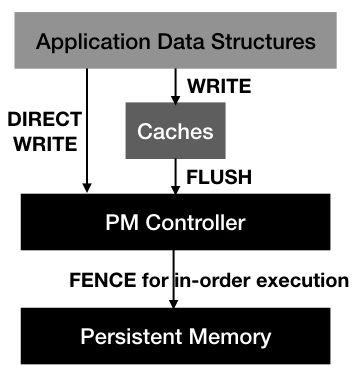
\includegraphics[width=\columnwidth]{figures/nvm-architecture.jpg}
    \caption{\emph{The architecture of Persitent Memory.}}
    \label{fig:architecture}
    \vspace{-0.3in}
\end{figure}


PM-CHECKER\footnote{https://github.com/SoujanyaPonnapalli/ASE-396-CourseProject}
models the architecture as shown in the Figure-\cite{fig-nvm-architecture}.

%\section{Desired Outcomes}


%\clearpage

% \nocite{*}
\bibliographystyle{is-unsrt}
%\bibliographystyle{ACM-Reference-Format}
\bibliography{ref}

\end{document}
